% (find-LATEX "2022-1-C3-notacao-de-fisicos.tex")
% (defun c () (interactive) (find-LATEXsh "lualatex -record 2022-1-C3-notacao-de-fisicos.tex" :end))
% (defun C () (interactive) (find-LATEXsh "lualatex 2022-1-C3-notacao-de-fisicos.tex" "Success!!!"))
% (defun D () (interactive) (find-pdf-page      "~/LATEX/2022-1-C3-notacao-de-fisicos.pdf"))
% (defun d () (interactive) (find-pdftools-page "~/LATEX/2022-1-C3-notacao-de-fisicos.pdf"))
% (defun e () (interactive) (find-LATEX "2022-1-C3-notacao-de-fisicos.tex"))
% (defun o () (interactive) (find-LATEX "2021-2-C3-notacao-de-fisicos.tex"))
% (defun u () (interactive) (find-latex-upload-links "2022-1-C3-notacao-de-fisicos"))
% (defun v () (interactive) (find-2a '(e) '(d)))
% (defun d0 () (interactive) (find-ebuffer "2022-1-C3-notacao-de-fisicos.pdf"))
% (defun cv () (interactive) (C) (ee-kill-this-buffer) (v) (g))
%          (code-eec-LATEX "2022-1-C3-notacao-de-fisicos")
% (find-pdf-page   "~/LATEX/2022-1-C3-notacao-de-fisicos.pdf")
% (find-sh0 "cp -v  ~/LATEX/2022-1-C3-notacao-de-fisicos.pdf /tmp/")
% (find-sh0 "cp -v  ~/LATEX/2022-1-C3-notacao-de-fisicos.pdf /tmp/pen/")
%     (find-xournalpp "/tmp/2022-1-C3-notacao-de-fisicos.pdf")
%   file:///home/edrx/LATEX/2022-1-C3-notacao-de-fisicos.pdf
%               file:///tmp/2022-1-C3-notacao-de-fisicos.pdf
%           file:///tmp/pen/2022-1-C3-notacao-de-fisicos.pdf
% http://angg.twu.net/LATEX/2022-1-C3-notacao-de-fisicos.pdf
% (find-LATEX "2019.mk")
% (find-CN-aula-links "2022-1-C3-notacao-de-fisicos" "3" "c3m221nf" "c3nf")
% (find-sh0 "cd ~/LUA/; cp -v Pict2e1.lua Pict2e1-1.lua Piecewise1.lua ~/LATEX/")
% (find-sh0 "cd ~/LUA/; cp -v Pict2e1.lua Pict2e1-1.lua Pict3D1.lua ~/LATEX/")

% «.defs»			(to "defs")
% «.title»			(to "title")
% «.exercicio-1»		(to "exercicio-1")
% «.exercicio-2»		(to "exercicio-2")
% «.truques-de-traducao»	(to "truques-de-traducao")
% «.truques-de-traducao-2»	(to "truques-de-traducao-2")
% «.miranda-ex.4.4-p.120»	(to "miranda-ex.4.4-p.120")
% «.miranda-ex.4.4-p.120-2»	(to "miranda-ex.4.4-p.120-2")
% «.exercicios-3-e-4»		(to "exercicios-3-e-4")
% «.dy-is-a-dep-var»		(to "dy-is-a-dep-var")
% «.variaveis-novas»		(to "variaveis-novas")
% «.exercicios-5-e-6»		(to "exercicios-5-e-6")
% «.derivadas-parciais-th»	(to "derivadas-parciais-th")
% «.derivadas-totais»		(to "derivadas-totais")
% «.exercicio-9»		(to "exercicio-9")
% «.exercicio-10»		(to "exercicio-10")
% «.exercicio-10-dicas»		(to "exercicio-10-dicas")
% «.exercicio-10-dicas-2»	(to "exercicio-10-dicas-2")
% «.piramide»			(to "piramide")
% «.piramide-2»			(to "piramide-2")
% «.low-poly»			(to "low-poly")
%   «.video-quadraticas»	(to "video-quadraticas")
%   «.video-cabos»		(to "video-cabos")
% «.regioes»			(to "regioes")
% «.regioes-2»			(to "regioes-2")
% «.exercicio-11»		(to "exercicio-11")
% «.exercicio-12»		(to "exercicio-12")
% «.exercicio-13»		(to "exercicio-13")
% «.barranco»			(to "barranco")
% «.exercicio-14»		(to "exercicio-14")
% «.f_barranco»			(to "f_barranco")
% «.exercicio-15»		(to "exercicio-15")
% «.exercicio-16»		(to "exercicio-16")
% «.derivada-direcional»	(to "derivada-direcional")
% «.gradiente»			(to "gradiente")
% «.fronteira»			(to "fronteira")
% «.funcoes-homogeneas»		(to "funcoes-homogeneas")
%
% «.djvuize»			(to "djvuize")



% <videos>
% Video (not yet):
% (find-ssr-links     "c3m221nf" "2022-1-C3-notacao-de-fisicos")
% (code-eevvideo      "c3m221nf" "2022-1-C3-notacao-de-fisicos")
% (code-eevlinksvideo "c3m221nf" "2022-1-C3-notacao-de-fisicos")
% (find-c3m221nfvideo "0:00")

\documentclass[oneside,12pt]{article}
\usepackage[colorlinks,citecolor=DarkRed,urlcolor=DarkRed]{hyperref} % (find-es "tex" "hyperref")
\usepackage{amsmath}
\usepackage{amsfonts}
\usepackage{amssymb}
\usepackage{pict2e}
\usepackage[x11names,svgnames]{xcolor} % (find-es "tex" "xcolor")
\usepackage{colorweb}                  % (find-es "tex" "colorweb")
%\usepackage{tikz}
%
% (find-dn6 "preamble6.lua" "preamble0")
%\usepackage{proof}   % For derivation trees ("%:" lines)
%\input diagxy        % For 2D diagrams ("%D" lines)
%\xyoption{curve}     % For the ".curve=" feature in 2D diagrams
%
\usepackage{edrx21}               % (find-LATEX "edrx21.sty")
\input edrxaccents.tex            % (find-LATEX "edrxaccents.tex")
\input edrx21chars.tex            % (find-LATEX "edrx21chars.tex")
\input edrxheadfoot.tex           % (find-LATEX "edrxheadfoot.tex")
\input edrxgac2.tex               % (find-LATEX "edrxgac2.tex")
%\usepackage{emaxima}              % (find-LATEX "emaxima.sty")
%
%\usepackage[backend=biber,
%   style=alphabetic]{biblatex}            % (find-es "tex" "biber")
%\addbibresource{catsem-slides.bib}        % (find-LATEX "catsem-slides.bib")
%
% (find-es "tex" "geometry")
\usepackage[a6paper, landscape,
            top=1.5cm, bottom=.25cm, left=1cm, right=1cm, includefoot
           ]{geometry}
%
\begin{document}

\catcode`\^^J=10
\directlua{dofile "dednat6load.lua"}  % (find-LATEX "dednat6load.lua")
%L dofile "Pict2e1.lua"              -- (find-LATEX "Pict2e1.lua")
%L dofile "Pict2e1-1.lua"            -- (find-LATEX "Pict2e1-1.lua")
%L dofile "Piecewise1.lua"           -- (find-LATEX "Piecewise1.lua")
%L dofile "Pict3D1.lua"              -- (find-LATEX "Pict3D1.lua")
%L Pict2e.__index.suffix = "%"
\pu
\def\pictgridstyle{\color{GrayPale}\linethickness{0.3pt}}
\def\pictaxesstyle{\linethickness{0.5pt}}
\def\pictnaxesstyle{\color{GrayPale}\linethickness{0.5pt}}
\celllower=3pt

% %L dofile "2021pict2e.lua"           -- (find-LATEX "2021pict2e.lua")
% %L Pict2e.__index.suffix = "%"
% \pu
% \def\pictgridstyle{\color{GrayPale}\linethickness{0.3pt}}
% \def\pictaxesstyle{\linethickness{0.5pt}}

% %L dofile "edrxtikz.lua"  -- (find-LATEX "edrxtikz.lua")
% %L dofile "edrxpict.lua"  -- (find-LATEX "edrxpict.lua")
% \pu

% «defs»  (to ".defs")
% (find-LATEX "edrx21defs.tex" "colors")
% (find-LATEX "edrx21.sty")

\def\u#1{\par{\footnotesize \url{#1}}}

\def\ddx{\frac{d}{dx}}
\def\ddy{\frac{d}{dy}}
\def\ddz{\frac{d}{dz}}

\def\pictnaxesstyle{\color{Gray}\linethickness{0.5pt}}
 
\def\drafturl{http://angg.twu.net/LATEX/2022-1-C3.pdf}
\def\drafturl{http://angg.twu.net/2022.1-C3.html}
\def\draftfooter{\tiny \href{\drafturl}{\jobname{}} \ColorBrown{\shorttoday{} \hours}}



%  _____ _ _   _                               
% |_   _(_) |_| | ___   _ __   __ _  __ _  ___ 
%   | | | | __| |/ _ \ | '_ \ / _` |/ _` |/ _ \
%   | | | | |_| |  __/ | |_) | (_| | (_| |  __/
%   |_| |_|\__|_|\___| | .__/ \__,_|\__, |\___|
%                      |_|          |___/      
%
% «title»  (to ".title")
% (c3m221nfp 1 "title")
% (c3m221nfa   "title")

\thispagestyle{empty}

\begin{center}

\vspace*{1.2cm}

{\bf \Large Cálculo 3 - 2022.1}

\bsk

Aula 10: ``notação de físicos''

\bsk

Eduardo Ochs - RCN/PURO/UFF

\url{http://angg.twu.net/2022.1-C3.html}

\end{center}

\newpage

{\bf Links}

Links pro livro do Thompson e pro PDF do semestre passado:

\ssk

{\footnotesize

\url{https://www.gutenberg.org/files/33283/33283-pdf.pdf}

% (c3m212nfp 1)
%    http://angg.twu.net/LATEX/2021-2-C3-notacao-de-fisicos.pdf
\url{http://angg.twu.net/LATEX/2021-2-C3-notacao-de-fisicos.pdf}

}

\ssk

Vou acrescentar mais material aqui depois!


\newpage

\vspace*{-1cm}
% (find-latexscan-links "C3" "thompson_p11+11")
% (find-latexscan-links "C3" "thompson_p11+12")
% (find-xpdf-page "~/LATEX/2022-1-C3/thompson_p11+11.pdf")
% (find-xpdf-page "~/LATEX/2022-1-C3/thompson_p11+12.pdf")
$
\hspace*{-0.5cm}
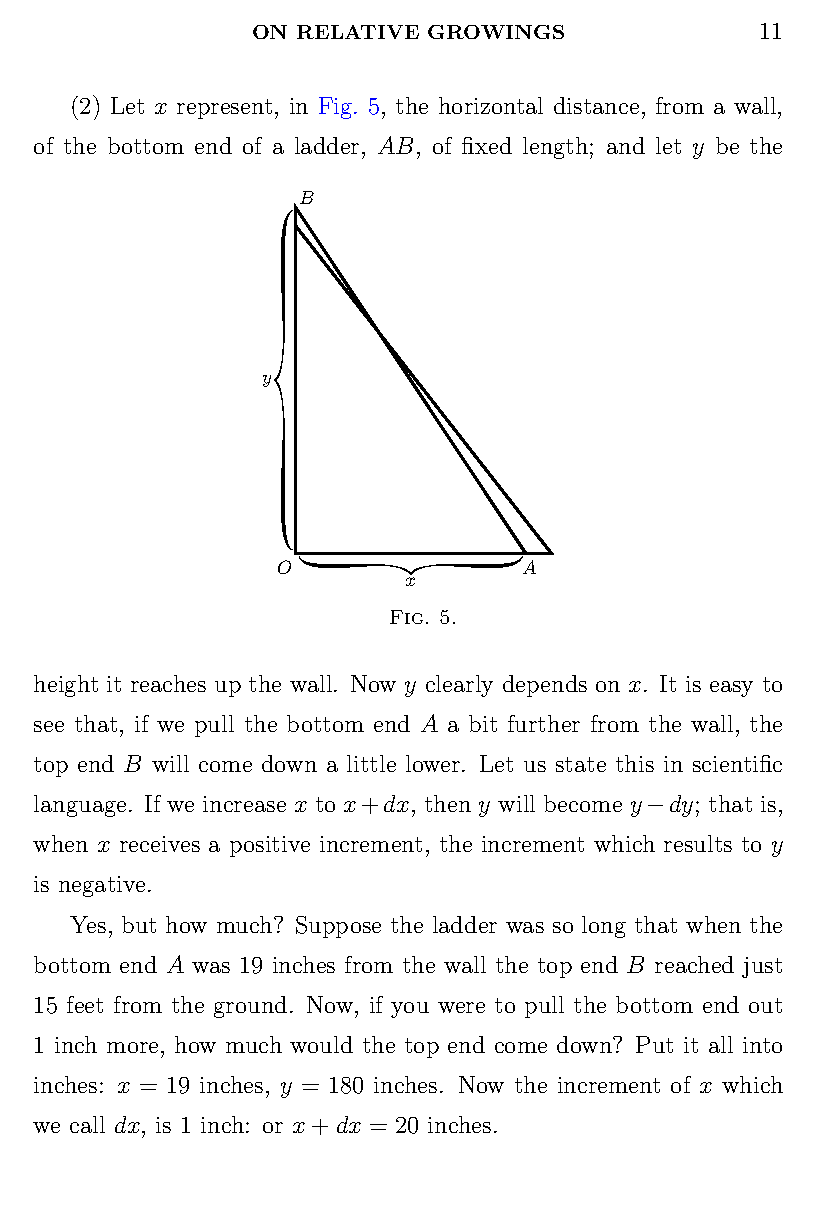
\includegraphics[width=6cm]{2022-1-C3/thompson_p11+11.pdf}
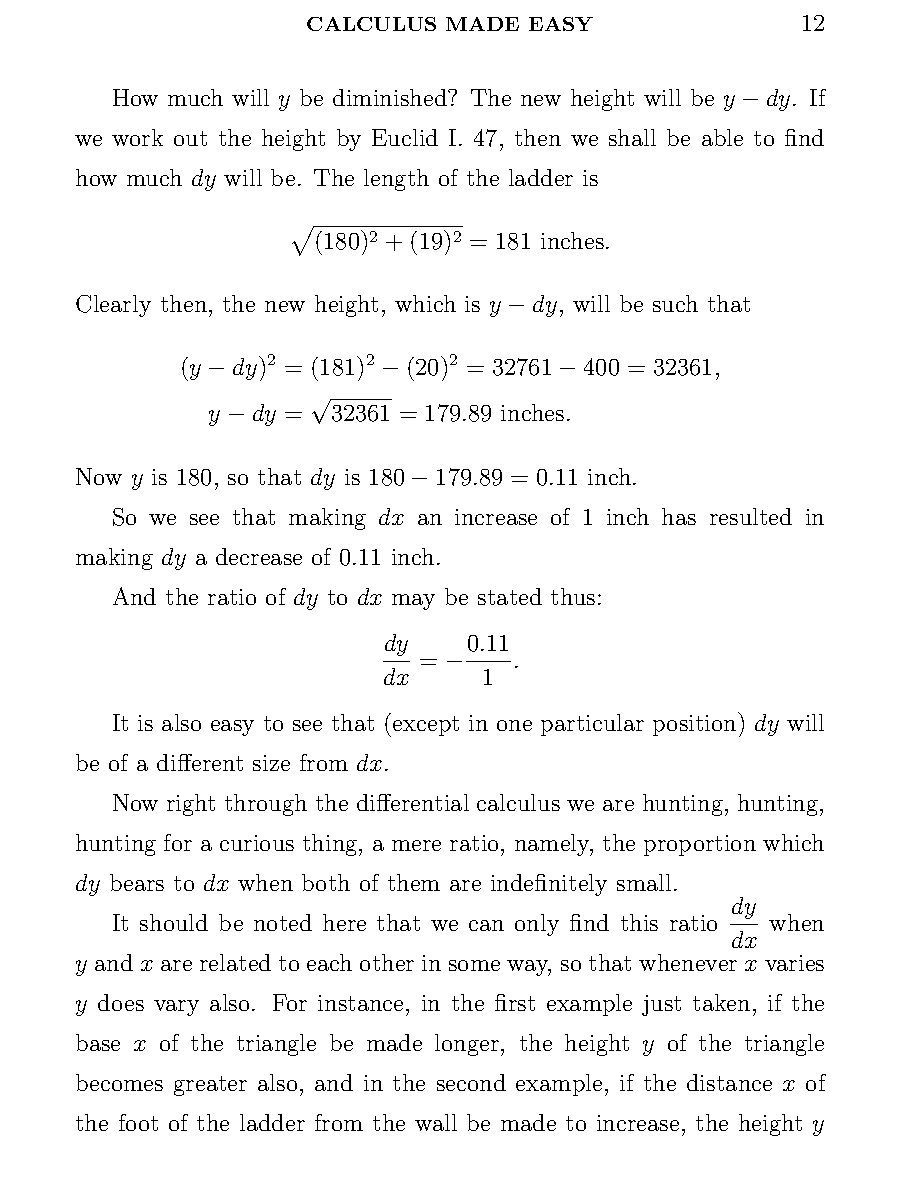
\includegraphics[width=6cm]{2022-1-C3/thompson_p11+12.pdf}
$

\newpage

%  _____                   _      _         _ 
% | ____|_  _____ _ __ ___(_) ___(_) ___   / |
% |  _| \ \/ / _ \ '__/ __| |/ __| |/ _ \  | |
% | |___ >  <  __/ | | (__| | (__| | (_) | | |
% |_____/_/\_\___|_|  \___|_|\___|_|\___/  |_|
%                                             
% «exercicio-1»  (to ".exercicio-1")
% (c3m221nfp 4 "exercicio-1")
% (c3m221nfa   "exercicio-1")

{\bf Exercício 1.}


\scalebox{0.5}{\def\colwidth{12cm}\firstcol{

    As contas à direita são uma versão um pouco modernizada das
    contas das páginas 11 e 12 do livro do Thompson. Repare que
    estamos usando $x_0$ e $y_0$ pros valores ``antes'' e `$x_1$ e
    $y_1$ pros valores ``depois'', e isso nos permite mencionar nas
    mesmas contas os valores de ``antes'' e de ``depois'' --- o
    Thompson precisa mantê-los em blocos de contas separados, e
    precisa de explicações em inglês pra dizer o que é o quê.

    \msk

    a) Numere as linhas das páginas 11 e 12 do Thompson e escreva ao
    lado de cada igualdade à direita a que linha do Thompson ela
    corresponde.

    \msk

    b) Faça uma versão da Fig.5 do Thompson que tenha proporções (um
    pouco) mais coerentes com os dados das contas dele, e que indique
    quais distâncias são $x_0$, $x_1$, $y_0$ e $y_1$. Faça tudo no
    olhômetro - não use régua.

    \msk

    c) Nas minhas contas eu usei o símbolo $ℓ$ pro comprimento da
    escada (``length''). Represente graficamente o círculo
    %
    $$\setofxyst{\sqrt{x^2+y^2}=ℓ}$$
    %
    e represente os pontos $(x_0,y_0)$ e $(x_1,y_1)$ nele. Faça tudo à
    mão sem régua, mas incluindo informações suficientes pro leitor
    entender o seu gráfico.

    \msk
    
    d) O $\frac{dy}{dx}$ do Thompson corresponde à derivada de qual
    função, em que ponto? Diga que função é essa, calcule a derivada
    dela, calcule na calculadora o valor da derivada dela no ponto
    certo, e compare o seu resultado com o valor do Thompson.



}\anothercol{

    \vspace*{-1cm}

    % (c3m212nfp 15 "escada-contas")
    % (c3m212nfa    "escada-contas")
    % (find-latexscan-links "C3" "20210806_silvanus_escada_contas")
    % (find-xpdf-page "~/LATEX/2021-1-C3/20210806_silvanus_escada_contas.pdf")
    $\begin{array}[t]{c}\\
    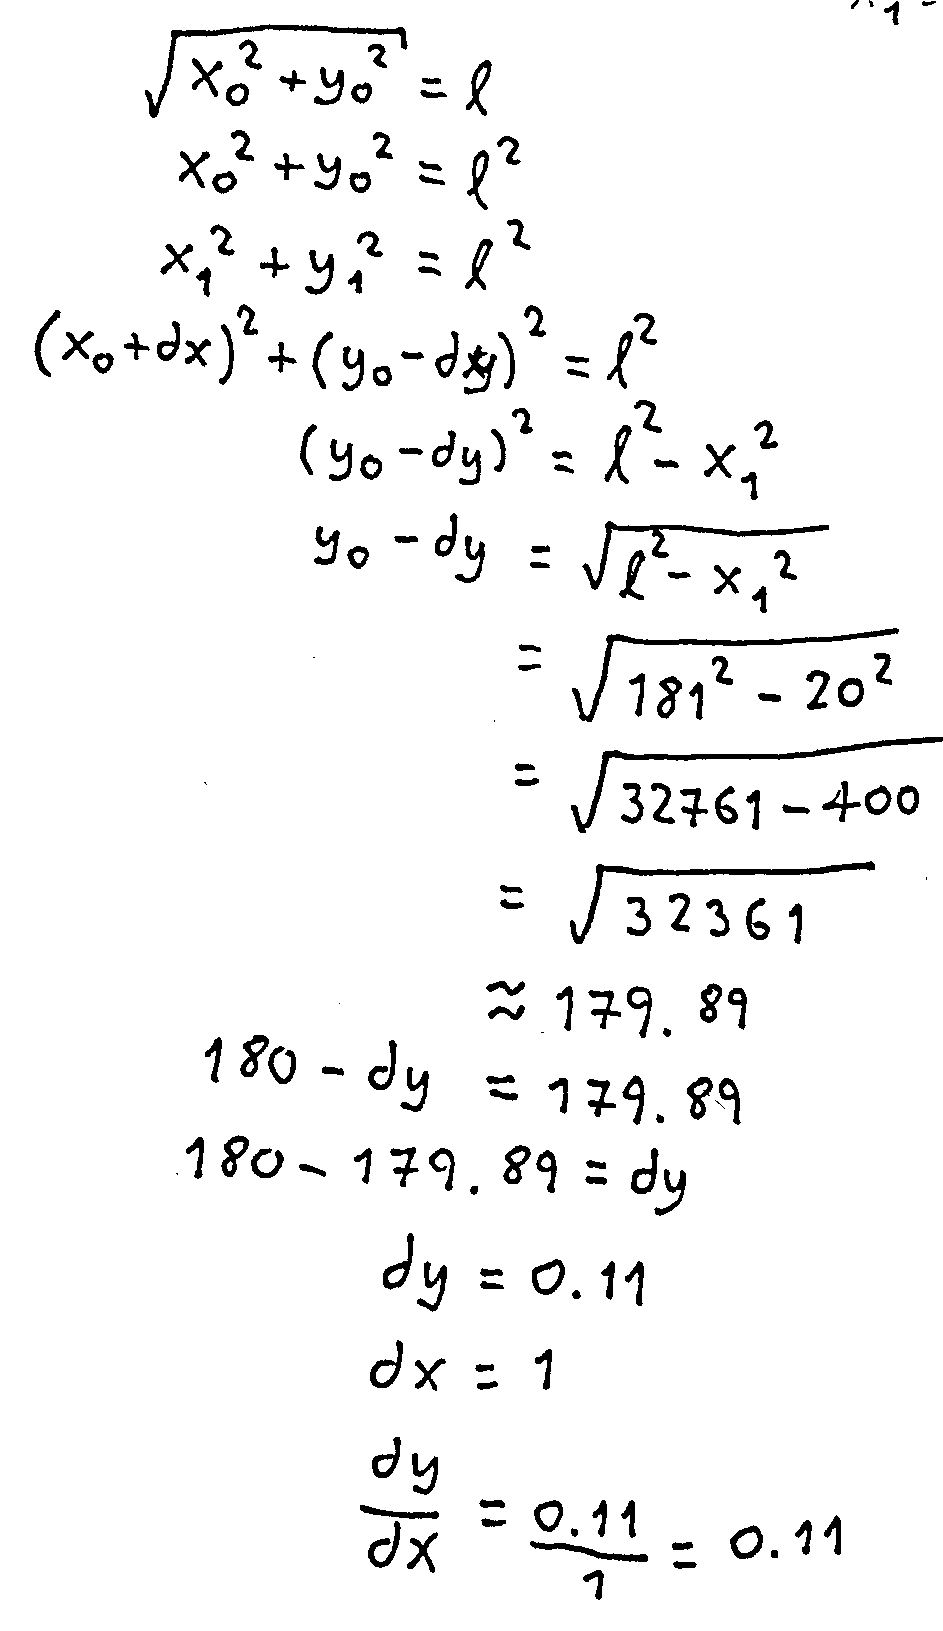
\includegraphics[height=13.5cm]{2021-1-C3/20210806_silvanus_escada_contas.pdf}
    \end{array}$

}}


\newpage

%  _____                   _      _         ____  
% | ____|_  _____ _ __ ___(_) ___(_) ___   |___ \ 
% |  _| \ \/ / _ \ '__/ __| |/ __| |/ _ \    __) |
% | |___ >  <  __/ | | (__| | (__| | (_) |  / __/ 
% |_____/_/\_\___|_|  \___|_|\___|_|\___/  |_____|
%                                                 
% «exercicio-2»  (to ".exercicio-2")
% (c3m221nfp 5 "exercicio-2")
% (c3m221nfa   "exercicio-2")

{\bf Exercício 2.}

\scalebox{0.8}{\def\colwidth{13cm}\firstcol{

Leia a seção 4.7 do livro do Daniel Miranda:

\ssk

{\scriptsize

% (find-books "__analysis/__analysis.el" "miranda")
% (find-dmirandacalcpage 117 "4.7 Aproximações Lineares e Diferencial")
% http://hostel.ufabc.edu.br/~daniel.miranda/calculo/calculo.pdf#page=117
\url{http://hostel.ufabc.edu.br/~daniel.miranda/calculo/calculo.pdf\#page=117}

}


\msk

Os livros mais modernos:

i) distinguem $dx$ e $Δx$,

ii) escrevem $y=f(x)$ ao invés de $y=y(x)$,

iii) evitam a convenção $x_1 = x_0+Δx$.

\bsk

a) Traduza o início da seção 4.7 do Miranda - até o fim

da página 118 - pra notação do Thompson. Dicas:
%
$$\begin{array}[c]{rcl}
  f(x) &≈& f(p)+f'(p)(x-p) \\
  L(x) &=& f(p)+f'(p)(x-p) \\
  \end{array}
  \;\;\;⇒\;\;\;
  \begin{array}[c]{rcl}
  f(x_1) &≈& f(x_0)+f'(x_0)Δx \\
  L(x_1) &=& f(x_0)+f'(x_0)Δx \\
  \end{array}
$$

e a função $L$ é exatamente a série de Taylor da função $f$ truncada
até grau 1... lembre que nós quase só vimos séries de Taylor no caso
em que $x_0$ era $0$, mas ficamos de ver depois o caso em que o
``ponto base'' não precisava mais ser 0...

%}\anothercol{
}}



\newpage

%  _____              _ 
% |_   _| __ __ _  __| |
%   | || '__/ _` |/ _` |
%   | || | | (_| | (_| |
%   |_||_|  \__,_|\__,_|
%                       
% «truques-de-traducao»  (to ".truques-de-traducao")
% (c3m221nfp 6 "truques-de-traducao")
% (c3m221nfa   "truques-de-traducao")

{\bf Alguns truques de tradução}

\scalebox{0.6}{\def\colwidth{14cm}\firstcol{

Truque 1: quando a gente escreve fórmulas ``com o mesmo formato''
perto uma da outra o leitor tende a ler a segunda ou como uma
\ColorRed{tradução} da primeira pra outra notação ou como um
\ColorRed{caso particular} da primeira...

\ssk

Isto aqui é uma tradução de duas das fórmulas da p.117 do D.\ Miranda
pra ``notação de físicos'':
%
$$\begin{array}[c]{rcl}
  f(x) &≈& f(p)+f'(p)(x-p) \\
  L(x) &=& f(p)+f'(p)(x-p) \\
  \end{array}
  \;\;\;⇒\;\;\;
  \begin{array}[c]{rcl}
  f(x_1) &≈& f(x_0)+f'(x_0)Δx \\
  L(x_1) &=& f(x_0)+f'(x_0)Δx \\
  \end{array}
$$

E isto aqui é um caso particular da primeira fórmula:
%
$$f(4.02) ≈ f(4) + f'(4)(4.02 - 4) \qquad\qquad (*)$$

Repare que a fórmula $(*)$ fica mais clara se escrevermos isto
explicitamente:
%
$$ x_1=4.02 \qquad x_0=4 $$

...e repare que se a gente tentar escrever isto aqui direto
%
$$\sqrt{4.02} ≈ \sqrt{4} + \sqrt{4}'(4.02 - 4)$$

fica confuso e péssimo --- não existe uma notação padrão pra derivada
de $\sqrt{x}$ em $x=4$!!! Aqui a gente TEM que usar um truque novo ---
a gente tem que dar um nome pra função $\sqrt{x}$. Por exemplo...

}\anothercol{
}}


\newpage

%  _____              _   ____  
% |_   _| __ __ _  __| | |___ \ 
%   | || '__/ _` |/ _` |   __) |
%   | || | | (_| | (_| |  / __/ 
%   |_||_|  \__,_|\__,_| |_____|
%                               
% «truques-de-traducao-2»  (to ".truques-de-traducao-2")
% (c3m221nfp 7 "truques-de-traducao-2")
% (c3m221nfa    "truques-de-traducao-2")

{\bf Alguns truques de tradução (2)}


\scalebox{0.75}{\def\colwidth{14cm}\firstcol{

Seja $f(x)=\sqrt{x} = x^{1/2}$.

Então $f'(x)=\frac12 x^{-1/2} = \frac12 \frac{1}{x^{1/2}} = \frac{1}{2\sqrt x}$, e
%
$$\begin{array}{rrcl}
    & f(4.02) &≈& f(4) + f'(4)(4.02 - 4) \\
  ⇒ \qquad
    & \sqrt{4.02} &≈& \sqrt{4} + \frac{1}{2\sqrt{4}}(4.02 - 4) \\
  \end{array}
$$

Repare que acima eu só fiz as subtituições $f(x):=\sqrt{x}$ e
$f'(x):=\frac{1}{2\sqrt{x}}$ --- eu acho que as contas mais mais
fáceis de entender se a gente fizer as substituições e as
simplificações em passos separados:

$$\begin{array}{rrcl}
    & f(4.02) &≈& f(4) + f'(4)(4.02 - 4) \\
  ⇒ \qquad
    & \sqrt{4.02} &≈& \sqrt{4} + \frac{1}{2\sqrt{4}}(4.02 - 4) \\
    &             &=& 2 + \frac{1}{4}(0.02) \\
    &             &=& 2 + 0.005 \\
    &             &=& 2.005 \\
    & \sqrt{4.02} &=& 2.004993765576342... \\
  \end{array}
$$

A última linha acima tem um `$=$' ao invés de um `$≈$', e eu calculei
o resultado dela com a calculadora.

}\anothercol{
}}


\newpage

% «miranda-ex.4.4-p.120»  (to ".miranda-ex.4.4-p.120")
% (c3m221nfp 8 "miranda-ex.4.4-p.120")
% (c3m221nfa   "miranda-ex.4.4-p.120")
% (find-books "__analysis/__analysis.el" "miranda")
% (find-dmirandacalcpage 117 "4.7 Aproximações Lineares e Diferencial")
% (find-dmirandacalcpage 120   "Exemplo 4.4" "Uma tigela")
% (find-dmirandacalctext 120   "Exemplo 4.4" "Uma tigela")

{\bf O exemplo 4.4 da página 120}

\scalebox{0.6}{\def\colwidth{9cm}\firstcol{

$$\begin{array}[t]{rrcl}
  &  V(x) &=& \frac{π}{3} (30x^2 - x^3) \\
  & V'(x) &=& \frac{π}{3} (60x - 3x^2) = π(20x-x^2) \\
  & V(x_1) &≈& V(x_0) + V'(x_0)(x_1-x_0) \\
  & V(x_1) - V(x_0) &≈& V'(x_0)(x_1-x_0) \\
  & V(x^*) - V(5) &≈& V'(5)(x^*-5) \\
    [10pt]
  & V(5) &=& \frac{π}{3} (30·5^2 - 5^3) \\
  &      &=& \frac{π}{3}625 \\
  & V'(5) &=& π(20·5-5^2) \\
  &       &=& 75π \\
    [10pt]
  & V(x^*) - V(5) &≈& V'(5)(x^*-5) \\
  & ΔV &≈& V'(5)Δx \\
  &    &=& 75πΔx \\
    [10pt]
  & V(x^*) - V(5) &≈& V'(5)(x^*-5) \\
  & V(x^*) &≈& V(5) + V'(5)(x^*-5) \\
  &        &=& \frac{π}{3}625 + 75πΔx \\
  \end{array}
$$

}\anothercol{

$$\begin{array}[t]{rrcl}
  & Δx &=& 0.1 \\
  ⇒
  & V(x^*) &=& \frac{π}{3}625 + 75π·0.1 \\
  &        &=& \frac{π}{3}625 + 75π·0.1 \\
  &        &≈& 654.5 + 23.56 \\
   [20pt]
  & Δx &=& ±0.1 \\
  ⇒
  & V(x^*) &=& \frac{π}{3}625 ± 75π·0.1 \\
  &        &=& \frac{π}{3}625 ± 75π·0.1 \\
  &        &≈& 654.5 ± 23.56 \\
  & V(x^*) &∈& [654.5 - 23.56, 654.5 + 23.56] \\
  \end{array}
$$

}}

\newpage

% «miranda-ex.4.4-p.120-2»  (to ".miranda-ex.4.4-p.120-2")
% (c3m221nfp 9 "miranda-ex.4.4-p.120-2")
% (c3m221nfa   "miranda-ex.4.4-p.120-2")

{\bf O exemplo 4.4 da página 120 (2)}


\scalebox{0.7}{\def\colwidth{15cm}\firstcol{

No exemplo 4.4 o D.\ Miranda faz as contas o mais rápido possível ---
porque ele quer que os leitores passem meia hora reescrevendo as
contas e checando os detalhes --- e ele usa um monte de truques de
físicos... por exemplo, ele fala em ``erro de medida'' e usa o `$±$'
no sentido que os físicos costumam usar: pra matemáticos a frase ``as
soluções de $(x-17)(x+23)=0$ são da forma $x=20±3$'' quer dizer que
$x=20-3$ ou $x=20+3$, mas pra físicos ``$x=20±3$'' quer dizer
$x∈[20-3,20+3]$...

\msk

Tem um monte de pessoas na turma que não fizeram Física.

\msk

Na página anterior eu escrevi as contas do exemplo 4.4 tentando fazer
com que elas ficassem bem fáceis de verificar por pessoas que não
fizeram Física. Eu fiz as contas com simplificações, como $V'(5)=75π$,
bem passo a passo, e deixei as contas com aproximações, como
$75π·0.1≈23.56$, pro final; além disso eu repeti algumas linhas, como
a que diz
%
$$V(x^*) - V(5) ≈ V'(5)(x^*-5)$$

várias vezes, e ao invés de tentar ver direto quais eram as
consequências de $Δx=±0.1$ eu comecei vendo as consequências de
$Δx=0.1$ e só depois passei pra $Δx=±0.1$... as contas com $Δx=±0.1$
são parecidas com as pra $Δx=0.1$, mas com alguns detalhes complicados
novos.

}\anothercol{
}}


\newpage

% «exercicios-3-e-4»  (to ".exercicios-3-e-4")
% (c3m221nfp 10 "exercicios-3-e-4")
% (c3m221nfa    "exercicios-3-e-4")

{\bf Exercício 3.}

Faça as contas do Exemplo 4.5 do D.\ Miranda ---

o que é sobre uma esfera --- de um jeito parecido

com o que eu usei nas contas do Exemplo 4.4 ---

que era sobre uma tigela...

\msk

Faça tudo BEM passo a passo e deixe os truques

``de físicos'' pros passos finais das contas.


\bsk
\bsk
\bsk

{\bf Exercício 4.}

Faça a mesma coisa pro Exemplo 4.6.




\newpage

% «dy-is-a-dep-var»  (to ".dy-is-a-dep-var")
% (c3m221nfp 11 "dy-is-a-dep-var")
% (c3m221nfa    "dy-is-a-dep-var")

{\bf ``$dy$ is always a dependent variable''}

Agora vamos ver como vários livros

lidam com esta idéia aqui:
%
$$\frac{dy}{dx} dx = dy$$

Repare que temos $\frac{dy}{dx}Δx ≈ Δy$ mas $\frac{dy}{dx}dx = dy$.

% {\scriptsize
% 
% % (find-books "__analysis/__analysis.el" "miranda")
% % (find-dmirandacalcpage 117 "4.7 Aproximações Lineares e Diferencial")
% % http://hostel.ufabc.edu.br/~daniel.miranda/calculo/calculo.pdf#page=117
% \url{http://hostel.ufabc.edu.br/~daniel.miranda/calculo/calculo.pdf\#page=117}
% 
% }

% (find-fline "~/2022.1-C3/")

O livro do Thomas explica isso bem melhor que o

livro do D.\ Miranda. Leia a definição de diferenciais

na p.225 do Thomas e entenda os exemplos 4 e 5

das páginas 225 e 227 dele:

\ssk

% (find-pdf-page "~/2022.1-C3/C3-quadros.pdf" 11)

{\scriptsize

% (find-books "__analysis/__analysis.el" "thomas")
% (code-pdf-page "thomas3738" "~/2022.1-C3/thomas_secoes_3.7_e_3.8.pdf")
% (code-pdf-text "thomas3738" "~/2022.1-C3/thomas_secoes_3.7_e_3.8.pdf")
% (find-thomas3738page)
% (find-thomas3738text)
% (find-thomas3738page (+ -211 225) "dy is always a dependent variable")
% (find-thomas3738text (+ -211 225) "dy is always a dependent variable")
% http://angg.twu.net/2022.1-C3/thomas_secoes_3.7_e_3.8.pdf#page=14
\url{http://angg.twu.net/2022.1-C3/thomas_secoes_3.7_e_3.8.pdf}

}

\newpage

% «variaveis-novas»  (to ".variaveis-novas")
% «exercicios-5-e-6»  (to ".exercicios-5-e-6")
% (c3m221nfp 12 "variaveis-novas")
% (c3m221nfa    "variaveis-novas")
% (c3m221nfp 12 "exercicios-5-e-6")
% (c3m221nfa    "exercicios-5-e-6")
% (c3m212nfp 19 "variaveis-novas")
% (c3m212nfa    "variaveis-novas")

{\bf O truque das variáveis novas}

\scalebox{0.7}{\def\colwidth{12cm}\firstcol{

% (find-books "__analysis/__analysis.el" "thompson")
% (find-sthompsonpage (+ 11  34) "VI. Sums, Differences, Products and Quotients")

No capítulo VI o Thompson calcula $\ddx((x^2 + c) + (ax^4 + b))$

organizando as contas mais ou menos desta forma:

$$\begin{array}{rcl}
  y &=& (x^2 + c) + (ax^4 + b) \\
  \frac{dy}{dx} &=& \frac{d((x^2+c) + (ax^4+b))}{dx} \\
                &=& \frac{d(x^2+c)}{dx} + \frac{d(ax^4+b)}{dx} \\
                &=& 2x + 4ax^3 \\
  \end{array}
$$

% (find-sthompsonpage (+ 11  66) "IX. Introducing a Useful Dodge")
% (find-sthompsontext (+ 11  66)     "INTRODUCING A USEFUL DODGE")

No capítulo IX -- ``Introducing a useful dodge'' --

o Thompson mostra como a gente pode simplificar contas

como essa introduzindo ``variáveis dependentes'' novas.

\bsk

{\bf Exercício 5.}

Entenda os exemplos (1)--(4) das páginas 66--68 do Thompson.

\bsk

% (find-sthompsonpage (+ 11  72)   "Exercises VI")
% (find-sthompsontext (+ 11  72)   "Exercises VI")

{\bf Exercício 6.}

Faça os exercícios (1)--(4) da página 72 do Thompson.

% (setq eepitch-preprocess-regexp "^")
% (setq eepitch-preprocess-regexp "^%T ")
%
%T  (eepitch-maxima)
%T  (eepitch-kill)
%T  (eepitch-maxima)
%T  (find-sthompsonpage (+ 11  72) "(1)")
%T y : sqrt(x^2 + 1);
%T diff(y, x);
%T  (find-sthompsonpage (+ 11  72) "(2)")
%T y : sqrt(x^2 + a^2);
%T diff(y, x);
%T  (find-sthompsonpage (+ 11  72) "(3)")
%T y : 1 / sqrt(a + x);
%T diff(y, x);
%T  (find-sthompsonpage (+ 11  72) "(4)")
%T y : a / sqrt(a - x^2);
%T diff(y, x);


\bsk

Links:

{\footnotesize

% https://www.gutenberg.org/files/33283/33283-pdf.pdf#page=45
\url{https://www.gutenberg.org/files/33283/33283-pdf.pdf\#page=45}

% https://www.gutenberg.org/files/33283/33283-pdf.pdf#page=83
\url{https://www.gutenberg.org/files/33283/33283-pdf.pdf\#page=83}

}

}}


\newpage

% «derivadas-parciais-th»  (to ".derivadas-parciais-th")
% (c3m221nfp 13 "derivadas-parciais-th")
% (c3m221nfa    "derivadas-parciais-th")
% (c3m212nfp 21 "derivadas-parciais-th")
% (c3m212nfa    "derivadas-parciais-th")
% (find-books "__analysis/__analysis.el" "thompson")
% (find-sthompsonpage (+ 11 172) "XVI. Partial Differentiation")

{\bf Derivadas parciais no Thompson}

Leia o início do capítulo XVI do Thompson ---

``XVI. Partial Differentiation'' --- da p.172 até p.174.

Entenda os exemplos (1) até (3) dele.

\bsk

{\bf Exercício 7.}

Faça os exercícios (1)--(5) das páginas 177 e 178 do Thompson.

Obs: o (6) precisa de gráficos 3D, vamos fazer ele depois.

\bsk

{\bf Exercício 8.}

\def\ppx{\frac{∂}{∂x}}
\def\ddt{\frac{d}{dt}}

Digamos que $F(x,y) = x^3y^4$, $g(t) = \sen t$, $h(t) = e^{2t}$.

Vamos usar esta notação aqui: $F_x = \frac{∂}{∂x}F$, $g_t=\frac{d}{dt}g$, etc.

\ssk

a) Calcule $\ddt F(g(t),h(t))$ usando ``notação de matemáticos''.

\ssk

b) Digamos que $x=g(t)$, $y=h(t)$, $z=F(x,y)$.

Calcule $\frac{d}{dt}z$ usando ``notação de físicos''.

\newpage

% «derivadas-totais»  (to ".derivadas-totais")
% (c3m221nfp 14 "derivadas-totais")
% (c3m221nfa    "derivadas-totais")
% (c3m212nfp 22 "derivadas-parciais-e-ts")
% (c3m212nfa    "derivadas-parciais-e-ts")

% (find-pdf-page "~/2022.1-C3/C3-quadros.pdf" 11)

{\bf Derivadas parciais e derivadas totais}

Digamos que $z = z(x,y)$ e $y = y(x)$.

\msk

Vamos começar com um caso bem concreto --- um que

eu usei em EDOs com variáveis separáveis em C2... link:
\ssk

{\footnotesize

% (c2m211edovsa "title")
% (c2m211edovsa "title" "Aula 25: EDOs com variáveis separáveis")
\url{http://angg.twu.net/LATEX/2020-2-C2-edovs.pdf}

}

\msk

O nosso caso bem concreto vai ser:

$z = z(x,y) = x^2 + y^2$,

$y = y(x) = \sqrt{1 - x^2}$.

quando nós \ColorRed{só} consideramos o $z = z(x,y) = x^2 + y^2$

as derivadas parciais de $z$ são $z_x = 2x$ e $z_y = 2y$,

mas quando \ColorRed{também} consideramos o $y = y(x) = \sqrt{1 - x^2}$

aí temos $z = z(x,y(x)) = x^2 + \sqrt{1-x^2}^2 = 1$, e $\frac{dz}{dx}=0$.

\msk

Esta derivada $\frac{dz}{dx} = \frac{d}{dx} z(x,y(x))$ é chamada de

\ColorRed{derivada total} de $z$ com relação a $y$.




\newpage

% «exercicio-9»  (to ".exercicio-9")
% (c3m212nfp 23 "exercicio-7")
% (c3m212nfa    "exercicio-7")

{\bf Exercício 9.}

Digamos que $z = z(x,y) = (x+2)(y+3)$

e que $y = y(x) = \sen x$.

a) Calcule $\frac{∂z}{∂x}$, $\frac{∂z}{∂y}$.

b) Calcule $\frac{dz}{dx}$.

c) Calcule $\frac{d}{dx}\frac{d}{dx}z$.

\msk

\ColorRed{Convenção:} quando uma expressão como $z_x$ puder

ser interpretada tanto como uma derivada parcial quanto

como uma derivada total o default é interpretá-la

como derivada parcial.


\newpage

% «exercicio-10»  (to ".exercicio-10")
% (c3m221nfp 99 "exercicio-10")
% (c3m221nfa    "exercicio-10")

% (c3m212nfp 24 "exercicio-8")
% (c3m212nfa    "exercicio-8")

{\bf Exercício 10.}

Digamos que $z=z(x,y)$ e $y=y(x)$.

(Isto é uma versão mais geral do exercício 9).

\ssk

a) Calcule $\frac{d}{dx}z$.

\ssk

b) Calcule $\frac{d}{dx}\frac{d}{dx}z$.

\bsk
\bsk

Dica: siga as dicas dos próximos dois slides,

e escreva as suas contas em várias notações

diferentes ``em paralelo''.


% (find-books "__analysis/__analysis.el" "thompson-gardner")
% (find-fline "~/books/__analysis/" "thompson_gardner__calculus_made_easy.pdf")
% (find-sthompsongpage (+ 9  15)   "interval")
% (find-sthompsongtext (+ 9  15)   "interval")
% (find-sthompsongpage (+ 9  15)   "did not use the modern")
% (find-sthompsongtext (+ 9  15)   "did not use the modern")
% (find-sthompsongpage (+ 9 129)   "FIG. 30")
% (find-sthompsongtext (+ 9 129)   "FIG. 30")
% 24-26,138


\newpage

% «exercicio-10-dicas»  (to ".exercicio-10-dicas")
% (c3m221nfp 17 "exercicio-10-dicas")
% (c3m221nfa    "exercicio-10-dicas")

{\bf Dicas pro exercício 10}

\def\parenarl#1{\left(\begin{array}{l} #1 \end{array}\right)}
\def\aname#1{[\mathsf{A#1}]}

\scalebox{0.7}{\def\colwidth{9cm}\firstcol{

Compare:
%
$$\begin{array}{rcll}
  \aname1 &=&
  \parenarl{
    \ddx f(g(h(x))) \\
    = f'(g(h(x))) \ddx g(h(x)) \\
    = f'(g(h(x))) g'(h(x)) h'(x) \\
  }
  \\[20pt]
  \aname2 &=&
  \parenarl{
    \ddx \sen(\cos(\tan(x))) \\
    = \sen'(\cos(\tan(x))) \ddx \cos(\tan(x)) \\
    = \sen'(\cos(\tan(x))) \cos'(\tan(x)) \tan'(x) \\
  }
  \\[20pt]
  \aname3 &=&
  \parenarl{
    \ddx w(z(y(x))) \\
    = w'(z(y(x))) \ddx z(y(x)) \\
    = w'(z(z(x))) z'(y(x)) y'(x) \\
  }
  \\[20pt]
  \aname4 &=&
  \parenarl{
    \ddx w(z(y(x))) \\
    = w_z(z(y(x))) \ddx z(y(x)) \\
    = w_z(z(z(x))) z_y(y(x)) y_x(x) \\
  }
  %
  \\[20pt]
  \aname5 &=&
  \parenarl{
    \ddx w \\
    = w_z \ddx z \\
    = w_z z_y y_x \\
  }
  &
  \hspace*{-2cm}
  \begin{array}{l}
  y = y(x) \\
  z = z(y) = z(y(x)) \\
  w = w(z) = w(z(y)) = w(z(y(z))) \\
  \end{array}
  \\
  \end{array}
$$

}\anothercol{
}}

\newpage

% «exercicio-10-dicas-2»  (to ".exercicio-10-dicas-2")
% (c3m221nfp 17 "exercicio-10-dicas")
% (c3m221nfa    "exercicio-10-dicas")

{\bf Dicas pro exercício 10 (cont.)}


\scalebox{0.65}{\def\colwidth{10cm}\firstcol{

O $\aname1$ é a versão em ``notação de matemáticos''.

O $\aname1$ é a versão mais geral.

O $\aname2$ é um caso particular do $\aname1$.

O $\aname3$ é uma ``versão renomeada'' do $\aname1$.

O $\aname4$ é uma ``versão abreviada'' do $\aname3$.

\msk

Toda vez que a gente tiver dúvidas sobre como fazer contas

numa notação como a do $\aname5$ a gente vai expandir

ele pra notação do $\aname4$, depois renomear as funções

``que têm nomes de variáveis'', como $y(x) \squigto f(x)$,

depois fazer as contas na ``notação de matemáticos'', e

depois voltar pra ``notação de físicos''...

\msk

Ou seja: se $y=y(x)$, $z=z(y)$ e $w=w(z)$,
%
$$\begin{array}{rl}
           & \ddx w = ? \\
  \squigto & \ddx w(z(y(x))) = ? \\
  \squigto & \ddx h(g(f(x))) = ? \\
  \end{array}
$$

}\anothercol{

e a gente tem que escrever os nomes

novos...por exemplo:
%
$$\hspace*{-2cm}
  \begin{array}{l}
  y=y(x)=h(x), \\
  z=z(y)=g(y), \\
  w=w(z)=f(z) \\
  \end{array}
$$

e aí a gente calcula $\ddx h(g(f(x)))$ e

depois traduz as contas de volta pra

``notação de físicos''.

\msk

Lembre que eu nunca vi esse método

de tradução explicado direito, então

o que está aqui é uma {\sl tentativa}

de explicá-lo...

\msk

Ah, e se a gente se perder nas contas

na notação do $\aname1$ a gente pode tentar

fazer um caso particular, como o $\aname2$,

e depois voltar pro $\aname1$...



}}



\newpage


%  ____  _                     _     _      
% |  _ \(_)_ __ __ _ _ __ ___ (_) __| | ___ 
% | |_) | | '__/ _` | '_ ` _ \| |/ _` |/ _ \
% |  __/| | | | (_| | | | | | | | (_| |  __/
% |_|   |_|_|  \__,_|_| |_| |_|_|\__,_|\___|
%                                           
% «piramide»  (to ".piramide")
% (c3m221nfp 19 "piramide")
% (c3m221nfa    "piramide")
% (find-pdf-page "~/2022.1-C3/C3-quadros.pdf" 15)

{\bf Uma pirâmide}

(A gente viu isto na aula de 2022may20.)

\ssk

O objetivo desta aula e das próximas é fazer vocês

aprenderem a olhar pra algo como isso aqui...

%L -- (find-angg "LUA/Pict2e1-1.lua" "Numerozinhos-test3")
%L Pict2e.bounds = PictBounds.new(v(-1,-1), v(9,9))
%L pyr = Numerozinhos.from(0, 0, [[
%L     0 0 0 0 0 0 0 0 0
%L     0 0 0 0 0 0 0 0 0
%L     0 0 1 1 1 1 1 0 0
%L     0 0 1 2 2 2 1 0 0
%L     0 0 1 2 3 2 1 0 0
%L     0 0 1 2 2 2 1 0 0
%L     0 0 1 1 1 1 1 0 0
%L     0 0 0 0 0 0 0 0 0
%L     0 0 0 0 0 0 0 0 0 ]])
%L pyr_spec  =   "(1,1)--(7,1)--(7,7)--(1,7)--(1,1)--(7,7) (1,7)--(7,1)"
%L pyr_spec2 = [[ (1,7)--(7,7)--(7,1)--(1,1)--(1,7)--(7,1)
%L                (1,1)--(2,2)  (3,3)--(7,7)
%L                (2,2)--(2,3)--(3,3)--(3,2)--(2,2)
%L                (2,3)--(3,2)
%L             ]]
%L pyr:topict(         ):sa("piramide"             ):output()
%L pyr:topict(pyr_spec ):sa("piramide com linhas"  ):output()
%L pyr:topict(pyr_spec2):sa("piramide com linhas 2"):output()
\pu
%$$\ga{piramide}
%  \qquad
%  \ga{piramide com linhas}
%  \qquad
%  \ga{piramide com linhas 2}
%$$
%
$$\ga{piramide}
$$

...e verem uma pirâmide.

\newpage

% «piramide-2»  (to ".piramide-2")
% (c3m221nfp 20 "piramide-2")
% (c3m221nfa    "piramide-2")

{\bf Uma pirâmide (2)}

\ssk

Note que isto é {\sl muito} diferente da noção de função de Cálculo
1... não estamos dizendo o domínio da função $F(x,y)$ do slide
anterior, não estamos dando uma fórmula pra ela, e só estamos dando o
valor dela em alguns pontos...

\ssk

A figura do slide anterior só define uma função se 1) a gente diz que
ela representa a função mais simples possível que assume aqueles
valores, 2) se todo mundo tem a mesma noção de ``função mais simples
possível'', e 3) se não estamos num caso ambíguo.

\ssk

Releia isto aqui, sobre ``adivinhar trajetórias'':

\ssk

{\footnotesize

% (c3m212vtp 7 "sobre-adivinhar-trajetorias")
% (c3m212vta   "sobre-adivinhar-trajetorias")
%    http://angg.twu.net/LATEX/2021-2-C3-vetor-tangente.pdf#page=7
\url{http://angg.twu.net/LATEX/2021-2-C3-vetor-tangente.pdf\#page=7}

}

\msk

No diagrama de numerozinhos do slide anterior o leitor precisa
``adivinhar'' que a superfície $z=F(x,y)$ é feita de pedaços de
planos.

\newpage

%  _                    ____       _       
% | |    _____      __ |  _ \ ___ | |_   _ 
% | |   / _ \ \ /\ / / | |_) / _ \| | | | |
% | |__| (_) \ V  V /  |  __/ (_) | | |_| |
% |_____\___/ \_/\_/   |_|   \___/|_|\__, |
%                                    |___/ 
%
% «low-poly»  (to ".low-poly")
% (c3m221nfp 21 "low-poly")
% (c3m221nfa    "low-poly")

% https://en.wikipedia.org/wiki/Low_poly
% https://upload.wikimedia.org/wikipedia/commons/f/fb/Dolphin_triangle_mesh.png

{\bf Low Poly}


\scalebox{0.55}{\def\colwidth{13cm}\firstcol{

Computadores preferem pensar que superfícies 3D são feitas de
triângulos --- veja o golfinho abaixo e a página da Wikipedia sobre
``Low Poly''--- mas humanos preferem imaginar que triângulos vizinhos
que estão no mesmo plano em $\R^3$ são grudados e viram polígonos mais
complicados... Além disso qualquer diagrama de numerozinhos pode ser
triangulado de vários jeitos, e humanos costumam achar que a
triangulação da pirâmide acima à direita é ``mais natural'' que a
triangulação de baixo...

\ssk

Assista o vídeo sobre ``funções quadráticas'' (a partir do 4:05) pra
entender como nós vamos usar diagramas de numerozinhos pra superfícies
que não precisam ser compostas de polígonos, e o vídeo sobre ``cabos
na diagonal'' pra entender essa história das triangulações ``mais
naturais''.

Links:

\ssk

{\scriptsize


\url{https://en.wikipedia.org/wiki/Low_poly}

\ssk

% «video-quadraticas»  (to ".video-quadraticas")
% (c3m211qa "video-1")
% (find-ssr-links     "c3m211q" "2021-1-C3-funcoes-quadraticas" "2noSv8hyNIk")
% (code-eevvideo      "c3m211q" "2021-1-C3-funcoes-quadraticas" "2noSv8hyNIk")
% (code-eevlinksvideo "c3m211q" "2021-1-C3-funcoes-quadraticas" "2noSv8hyNIk")
% (find-c3m211qvideo "0:00")
\url{http://www.youtube.com/watch?v=2noSv8hyNIk}

\url{http://angg.twu.net/eev-videos/2021-1-C3-funcoes-quadraticas.mp4}

\ssk

% «video-cabos»  (to ".video-cabos")
% (c3m212dna          "video-diagonal")
% (find-ssr-links     "c3cd" "2021-2-c3-cabos-na-diagonal" "nxsIK0tPWAI")
% (code-eevvideo      "c3cd" "2021-2-c3-cabos-na-diagonal" "nxsIK0tPWAI")
% (code-eevlinksvideo "c3cd" "2021-2-c3-cabos-na-diagonal" "nxsIK0tPWAI")
% (find-c3cdvideo "0:00")
\url{http://www.youtube.com/watch?v=nxsIK0tPWAI}

\url{http://angg.twu.net/eev-videos/2021-2-c3-cabos-na-diagonal.mp4}


}

\bsk

% (find-latexscan-links "C3" "Dolphin_triangle_mesh")
% (find-xpdf-page "~/LATEX/2022-1-C3/Dolphin_triangle_mesh.pdf")
$$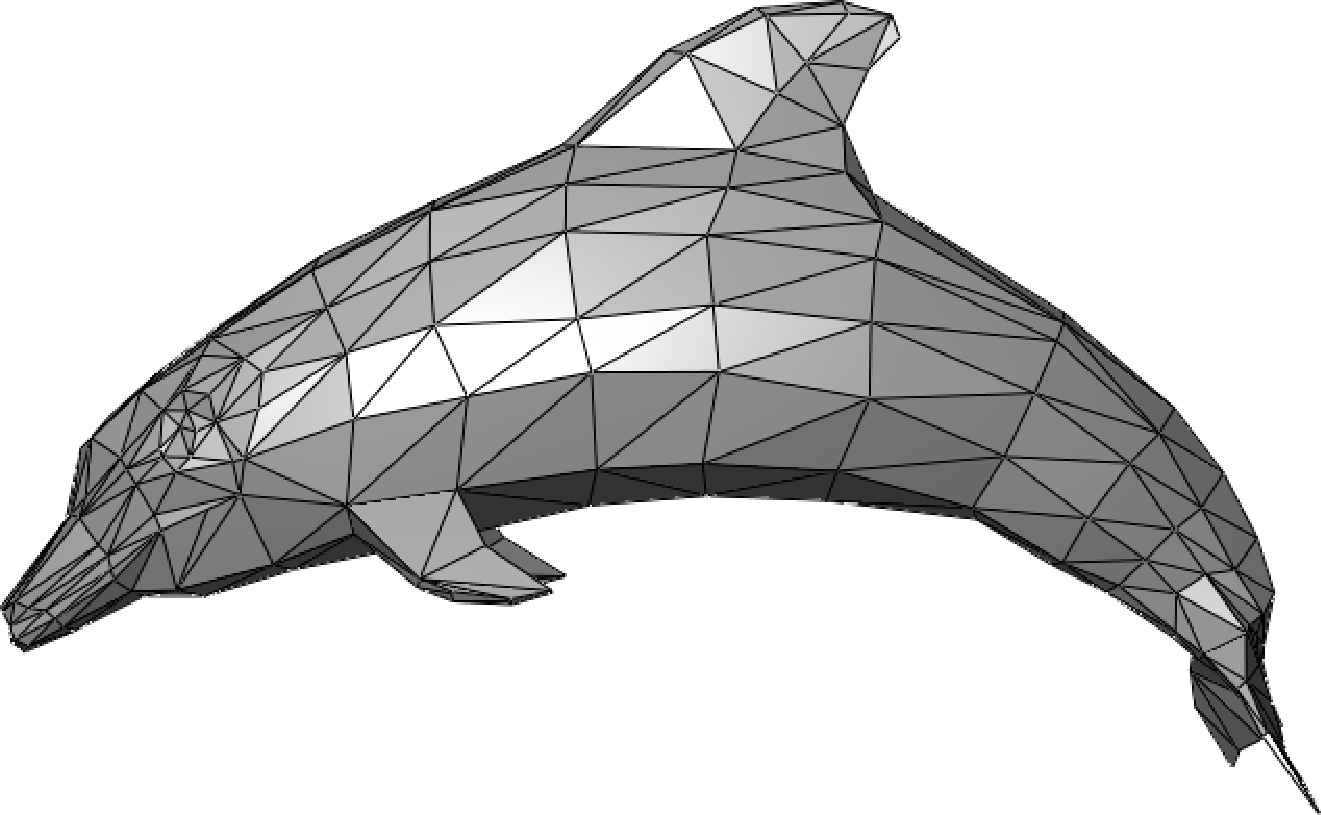
\includegraphics[width=5cm]{2022-1-C3/Dolphin_triangle_mesh.pdf}$$


}\anothercol{

\vspace*{0cm}

$\hspace*{1cm}
 \scalebox{1.25}{$
 \begin{array}{c}
 \ga{piramide com linhas} \\ \\
 \ga{piramide com linhas 2}
 \end{array}
 $}
$

}}

% (find-pdf-page "~/2022.1-C3/C3-quadros.pdf" 15)

\newpage

%  ____            _                 
% |  _ \ ___  __ _(_) ___   ___  ___ 
% | |_) / _ \/ _` | |/ _ \ / _ \/ __|
% |  _ <  __/ (_| | | (_) |  __/\__ \
% |_| \_\___|\__, |_|\___/ \___||___/
%            |___/                   
%
% «regioes»  (to ".regioes")
{\bf Regiões}

No próximo exercício vamos considerar

que o plano está divido nestas 5 regiões,

que vamos chamar de $N$, $W$, $E$, $S$, e $B$ ---

faces Norte, Oeste, Leste, Sul e ``base''...

$$\ga{piramide com linhas}
$$

% (find-pdf-page "~/2022.1-C3/C3-quadros.pdf" 16)

\newpage

%  ____            _                   ____  
% |  _ \ ___  __ _(_) ___   ___  ___  |___ \ 
% | |_) / _ \/ _` | |/ _ \ / _ \/ __|   __) |
% |  _ <  __/ (_| | | (_) |  __/\__ \  / __/ 
% |_| \_\___|\__, |_|\___/ \___||___/ |_____|
%            |___/                           
%
% «regioes-2»  (to ".regioes-2")
{\bf Regiões (2)}

%L Pict2e.bounds = PictBounds.new(v(0,0), v(6,6))
%L spec = "(0,2)--(2,2)--(4,4)--(6,4)"
%L linhas = PwSpec.from(spec):topict():prethickness("2pt")
%L linhas:pgat("pgatc"):preunitlength("7.5pt"):sa("Regioes 2"):output()
\pu

\def\fcases#1#2#3{
  \begin{cases}
     2 & \text{quando $#1$}, \\
     x & \text{quando $#2$}, \\
     4 & \text{quando $#3$} \\
  \end{cases}}

\def\pyrcases{
  \begin{cases}
     F_B(x,y) & \text{quando $(x,y)∈B$}, \\
     F_N(x,y) & \text{quando $(x,y)∈N$}, \\
     F_W(x,y) & \text{quando $(x,y)∈W$}, \\
     F_E(x,y) & \text{quando $(x,y)∈E$}, \\
     F_S(x,y) & \text{quando $(x,y)∈S$}, \\
  \end{cases}}


\scalebox{0.5}{\def\colwidth{13.5cm}\firstcol{

    As definições do $f_1, f_2, \ldots, f_5$ à direita definem a mesma
    função, e a definição do $f_5(x)$ é uma tradução ``pra notação com
    `$∈$'s\,'' da definição do $f_4(x)$...

    \msk

    Muitos matemáticos --- e livros, como por exemplo os do Guidorizzi
    --- consideram que as definições do $f_4(x)$ e do $f_5(x)$ são
    ruins porque as condições, ou ``regiões'', depois dos ``quando''s
    não são disjuntas, e aí essas definições ``só fazem sentido'' se a
    gente mostrar que quando $x∈(-∞,2]∩[2,4]$ temos $2=x$, e que
    quando $x∈[2,4]∩[4,-∞)$ temos $x=4$...

    \msk

    A definição $f_1(x)$ por um gráfico nos permite pular certos
    detalhes. É ``óbvio'' que ela corresponde a uma definição por
    casos com três casos diferentes, mas com a definição pelo gráfico
    a gente não precisa definir se o ponto $x=2$ pertence à primeira
    região ou à segunda, e nem se o ponto $x=4$ pertence à segunda
    região ou à terceira...

    \msk

    Dá pra gente definir a pirâmide do slide anterior ``de um jeito
    que deixaria o Guidorizzi feliz'' por uma definição por casos como
    a definição do $F_P(x)$ à direita, em que cada uma das funções
    $F_B, F_N, F_W, F_E, F_S$ é um ``plano'', isto é, é da forma
    $a + bx + cy$, e os conjuntos $B, N, W, E, S$ são descritos
    formalmente de jeitos como este aqui...
    %
    $$S \;\; = \;\; \setofxyst{x≥y, \; 1≤y, \; x+y≤8}$$

    Dê uma olhada nos slides 6 e 7 daqui:

    \ssk

    {\footnotesize

      % (c2m221isp 6 "exercicio-2")
      % (c2m221isa   "exercicio-2")
      % http://angg.twu.net/LATEX/2022-1-C2-infs-e-sups.pdf#page=6
      \url{http://angg.twu.net/LATEX/2022-1-C2-infs-e-sups.pdf\#page=6}

    }

    Daqui a algumas aulas nós vamos fazer um monte de exercícios de
    traduzir entre notação de conjuntos e representações gráficas ---
    nós vamos precisar disso pra entender conjuntos abertos em
    fechados em $\R^2$ --- mas por enquanto nós vamos definir regiões
    do plano por figuras.

}\anothercol{

\vspace*{0cm}

$
  \begin{array}{rcl}
  f_1(x) &=& \ga{Regioes 2} \\
  f_2(x) &=& \fcases{x<2}{2≤x≤4}{4<x} \\
  f_3(x) &=& \fcases{x≤2}{2<x<4}{4≤x} \\
  f_4(x) &=& \fcases{x≤2}{2≤x≤4}{4≤x} \\
  f_5(x) &=& \fcases{x∈(-∞,2]}{x∈[2,4]}{x∈[4,+∞)} \\
  \\
  F_P(x) &=& \pyrcases \\
  \end{array}
$

}}

\newpage

% «exercicio-11»  (to ".exercicio-11")
% (c3m221nfp 24 "exercicio-11")
% (c3m221nfa    "exercicio-11")
% (find-pdf-page "~/2022.1-C3/C3-quadros.pdf" 16)

{\bf Exercício 11.}

Faça o diagrama de numerozinhos de cada uma das superfícies

$z=F(x,y)$ abaixo. Desenhe os numerozinhos nos pontos com

$x,y∈\{0,1,2,3,4\}$ --- ou seja, 25 numerozinhos em cada item.

\msk

a) $F(x,y) = 2x$

b) $F(x,y) = 3y$

c) $F(x,y) = 2x + 3y$

d) $F(x,y) = 10 + 2x + 3y$

\bsk

% «exercicio-12»  (to ".exercicio-12")
% (c3m221nfp 24 "exercicio-12")
% (c3m221nfa    "exercicio-12")

{\bf Exercício 12.}

Mostre que se $z = F(x,y)$ é um plano com equação

$F(x,y) = a + bx + cy$ então isto aqui vale:
%
$$∀(x_0,y_0),(x_1,y_1)∈\R^2. \; Δz = bΔx + cΔy.$$

\newpage

% «exercicio-13»  (to ".exercicio-13")
% (c3m221nfp 25 "exercicio-13")
% (c3m221nfa    "exercicio-13")

{\bf Exercício 13.}


\scalebox{0.8}{\def\colwidth{12cm}\firstcol{

A pirâmide dos slides anteriores pode ser descrita formalmente

por uma definição por casos como esta aqui,
%
$$\scalebox{0.7}{$
  z \;\;=\;\;  F_P(x) \;\;=\;\; \pyrcases
  $}
$$

onde cada um dos $F_R(x,y)$, onde $R$ é $B, N, E, W$ ou $S$, é uma
equação de um plano --- ou seja, é ``da forma $a+bx+cy$''. Descubra
quais são estas equações de planos e escreva a sua resposta neste
formato aqui, mas com os números certos:
%
$$\scalebox{0.8}{$
  \begin{array}{rcl}
  F_B(x,y) &=& 2+3x+4y \\
  F_N(x,y) &=& 5+6x+7y \\
  F_W(x,y) &=& 8+9x+10y \\
  F_E(x,y) &=& 11+12x+13y \\
  F_S(x,y) &=& 14+15x+16y \\
  \end{array}
  $}
$$

}\anothercol{
}}


\newpage

% «barranco»  (to ".barranco")
% (c3m221nfp 26 "barranco")
% (c3m221nfa    "barranco")
% (find-angg "GNUPLOT/barranco.dem")

% «exercicio-14»  (to ".exercicio-14")
% (c3m221nfp 26 "exercicio-14")
% (c3m221nfa    "exercicio-14")

{\bf Exercício 14 (``barranco'').}

No exemplo da pirâmide a gente começou com um diagrama de numerozinhos
e aí encontrou um modo de dividir o plano em 5 regiões que fazia com
que todos os numerozinhos numa mesma região ficassem no mesmo plano.
Faça a mesma coisa com o diagrama de numerozinhos abaixo --- você vai
precisar de pelo menos 6 regiões.
%
%L Pict2e.bounds = PictBounds.new(v(-1,-1), v(9,9))
%L barranco = Numerozinhos.from(0, 0, [[
%L     4 4 4 4 4 4 4 4 4
%L     4 4 4 4 4 4 4 4 4
%L     3 3 3 3 4 4 4 4 4
%L     2 2 2 2 3 4 4 4 4
%L     1 1 1 1 2 3 4 4 4
%L     0 0 0 0 1 2 3 4 4
%L     0 0 0 0 0 1 2 2 2
%L     0 0 0 0 0 0 1 1 1
%L     0 0 0 0 0 0 0 0 0 ]])
%L barranco_spec = [[
%L     (0,7)--(3,7)--(7,3)--(8,3)
%L     (3,7)--(3,3)  (7,3)--(6,2)  (6,0)--(6,2)--(8,2)
%L     (0,3)--(3,3)--(6,0)--(8,0)  ]]
%L barranco:topict(             ):sa("barranco"):output()
%L barranco:topict(barranco_spec):sa("barranco com linhas"):output()
\pu
$$\ga{barranco}
  %\quad
  %\ga{barranco com linhas}
$$


% «f_barranco»  (to ".f_barranco")
% (setq eepitch-preprocess-regexp "^")
% (setq eepitch-preprocess-regexp "^%T ")
%
%T  (eepitch-lua51)
%T  (eepitch-kill)
%T  (eepitch-lua51)
%T pr = function (f)
%T     for y=8,0,-1 do
%T       for x=0,8 do
%T         printf("%d ", f(x,y))
%T       end
%T       print()
%T     end
%T   end
%T MAX = function (f, g)
%T     return function (x,y) return max(f(x,y), g(x,y)) end
%T   end
%T MIN = function (f, g)
%T     return function (x,y) return min(f(x,y), g(x,y)) end
%T   end
%T trAF = function (f) return MAX(MIN(fA, f), fF) end
%T fA = Code.ve(" x,y => 4     ")
%T fB = Code.ve(" x,y => y-3   ")
%T fC = Code.ve(" x,y => x+y-6 ")
%T fD = Code.ve(" x,y => y     ")
%T fE = Code.ve(" x,y => 2*y-2 ")
%T fF = Code.ve(" x,y => 0     ")
%T pr(fA)
%T pr(fB)
%T pr(fF)
%T pr(trAF(fB))
%T pr(trAF(fC))
%T pr(trAF(fD))
%T pr(trAF(fE))
%T fDE   = trAF(MAX(fD,  fE))
%T fBC   = trAF(MAX(fB,  fC))
%T fBCDE = trAF(MIN(fBC, fDE))
%T pr(fDE)
%T pr(fBC)
%T pr(fBCDE)

$\def\B{\ga{barranco}}
  \scalebox{0.6}{$
  \begin{array}{cccc}
  \B & \B & \B & \B \\
  \B & \B & \B & \B \\
  \B & \B & \B & \B \\
  \end{array}
  $}
$




\newpage

% «exercicio-15»  (to ".exercicio-15")
% (c3m221nfp 28 "exercicio-15")
% (c3m221nfa    "exercicio-15")

{\bf Exercício 15.}

\scalebox{0.7}{\def\colwidth{11cm}\firstcol{

Lembre que em planos a fórmula da aproximação linear
%
$$\begin{array}{rcl}
  F(x_0+Δx,y_0+Δy) &≈& F(x_0,y_0) \\
                   &+& F_x(x_0,y_0) Δx \\
                   &+& F_y(x_0,y_0) Δy \\
  \end{array}
$$

dá resultados exatos...

\bsk
Seja $z=F(x,y)$ a função que dá a superfície da pirâmide da figura à
direita. Descubra os valores de:

\def\TC#1{\begin{tabular}[t]{c}#1\end{tabular}}

\TC{a) F(1.5, 3) \\
    b) F(1.1, 3) \\
    c) F(5.1, 3) \\
    d) F(5.1, 2) \\
   }
\quad
\TC{e) F(5.2, 2.3) \\
    f) F(5.2, 1.9) \\
    g) F(3.1, 2.1) \\
    h) F(2.9, 1.9) \\
   }

\msk

Tente fazer as contas de cabeça.

Se você se enrolar faça as contas todas explicitamente, e use os
``truques de tradução'' das páginas 6 e 7 pra fazer as contas da forma
mais clara possível... depois esconda as suas contas e tente obter
todos os resultados de novo de cabeça.



}\anothercol{

\vspace*{0.7cm}

$\ga{piramide com linhas}
$

}}





\newpage

% «exercicio-16»  (to ".exercicio-16")
% (c3m221nfp 29 "exercicio-16")
% (c3m221nfa    "exercicio-16")

{\bf Exercício 16.}

\scalebox{0.7}{\def\colwidth{11cm}\firstcol{

Seja $z=F(x,y)$ a função que dá a superfície da pirâmide com duas
faces extras da figura à direita. Descubra os valores de:

\msk

\def\TC#1{\begin{tabular}[t]{c}#1\end{tabular}}

\TC{a) F(2.1, 2.1) \\
    b) F(2.5, 2.5) \\
    c) F(2.6, 2.6) \\
   }

\msk

fazendo as contas de cabeça.



}\anothercol{

\vspace*{0.25cm}

$\ga{piramide com linhas 2}
$

}}



\newpage

% «derivada-direcional»  (to ".derivada-direcional")
% (c3m221nfp 30 "derivada-direcional")
% (c3m221nfa    "derivada-direcional")
% (c3m212qp 32 "derivada-direcional")
% (c3m212qa    "derivada-direcional")
% (find-LATEXgrep "grep --color=auto -niH --null -e direcional *.tex")

{\bf Derivada direcional (Bortolossi)}


\scalebox{0.7}{\def\colwidth{9cm}\firstcol{

% (find-bortolossi8page (+ -290 291) "8. Derivadas direcionais e o vetor gradiente")
% (find-bortolossi8page (+ -290 296)   "Definição 8.1. (Derivada direcional)")
% (find-bortolossi8page (+ -290 298) "8.2. O vetor gradiente")
% (find-bortolossi8page (+ -290 302)   "direção de maior crescimento")

O Bortolossi define a derivada direcional

deste jeito, na p.296 do capítulo 8 dele:

$$\frac{∂f}{∂𝐛v}(𝐛p) =
  \lim_{t→0} \frac{ f(𝐛p + t·𝐛v) - f(𝐛p) }{t}
$$

\msk

Digamos que $f:\R^2→\R$, que os argumentos da $f$

se chamem $x$ e $y$, que $𝐛p=(x_0,y_0)$, que o vetor $𝐛v$

seja $(α,β)$, e que $z=z(x,y)=f(x,y)$.


\bsk

{\bf Exercício 17.}

Seja $f(x,y) = z(x,y) = F(x,y)$, onde $F(x,y)$ é a pirâmide do
exercício 15 (figura à direita).

Sejam $𝐛p = (x_0,y_0) = (2,3)$ e $𝐛v = \VEC{α,β} = \VEC{2,0}$.

Calcule $\frac{ f(𝐛p + t·𝐛v) - f(𝐛p) }{t}$ para os seguintes valores
de $t$:

\msk

\def\TC#1{\begin{tabular}[t]{l}#1\end{tabular}}

\TC{a) $t=1$ \\
    b) $t=2$ \\
    c) $t=3$ \\
    d) $t=1/2$ \\
    }
\quad
\TC{e) $t=1/4$ \\
    f) $t=-1$ \\
    g) $t=-1/2$ \\
    h) $t=-1/4$ \\
   }



}\anothercol{

\vspace*{0.7cm}

$\ga{piramide com linhas}
$

\bsk

{\bf Exercício 18.}

A partir do que você obteve no

exercício 17, qual você acha que

deve ser o valor de $\frac{∂f}{∂\VEC{2,0}}((2,3))$?

\bsk

{\bf Exercício 19.}

...e o valor de $\frac{∂f}{∂\VEC{1,0}}((2,3))$?

}}


\newpage

% «gradiente»  (to ".gradiente")
% (c3m221nfp 31 "gradiente")
% (c3m221nfa    "gradiente")

{\bf O gradiente}

% (c3m221mt1p 2 "defs-miniteste")
% (c3m221mt1a   "defs-miniteste")
%
%L -- (find-angg "LUA/Pict2e1-1.lua" "Numerozinhos-test3")
%L Pict2e.bounds = PictBounds.new(v(-1,-1), v(11,11))
%L pyr = Numerozinhos.from(0, 0, [[
%L     0 0 0 0 0 0 0 0 0 0 0 0
%L     0 0 0 0 0 0 0 0 0 0 0 0
%L     0 0 0 0 0 0 0 1 0 0 0 0
%L     0 0 0 0 0 0 1 2 0 0 0 0
%L     0 0 0 0 0 1 2 3 1 0 0 0
%L     0 0 0 0 1 2 3 4 2 0 0 0
%L     0 0 0 1 2 3 4 5 3 1 0 0
%L     0 0 1 2 3 4 5 6 4 2 0 0
%L     0 0 0 0 1 2 3 4 2 0 0 0
%L     0 0 0 0 0 0 1 2 0 0 0 0
%L     0 0 0 0 0 0 0 0 0 0 0 0
%L     0 0 0 0 0 0 0 0 0 0 0 0 ]])
%L pyr_spec  = "(1,4)--(7,10)--(10,4)--(7,1)--(1,4) (1,4)--(10,4) (7,1)--(7,10)"
%L pyr:topict(pyr_spec ):sa("piramide MT1 com linhas"):output()
\pu

\scalebox{0.65}{\def\colwidth{12cm}\firstcol{

Obs: esse exercício aqui vai ser totalmente reescrito depois!

Leia a definição de gradiente na página p.298 do capítulo 8

do Bortolossi. Tente entendê-la usando as dicas abaixo.

\msk

Se $F:\R^2→\R$, então:

\ssk

a) $\frac{∂F}{∂x_1}(x_0,y_0) = \frac{∂F}{∂x}(x_0,y_0) = F_x(x_0,y_0)$,

\ssk

b) $\frac{∂F}{∂x}(x_0,y_0) = \frac{∂F}{∂\VEC{1,0}}(x_0,y_0)$,

\ssk

c) $\frac{∂F}{∂y}(x_0,y_0) = \frac{∂F}{∂\VEC{0,1}}(x_0,y_0)$

\ssk

d) $∇F = \VEC{F_x, F_y}$

\bsk

{\bf Exercício 20.}

a) Usando a $F$ da pirâmide mais simples, calcule:

$∇F(2,4), ∇F(4,2), ∇F(6,4), ∇F(4,6)$.

\msk

b) Represente graficamente $(x_0,y_0) + ∇F(x_0,y_0)$ para

estes valores de $(x_0,y_0)$: $(2,4), (4,2), (6,4), (4,6)$.

\msk

c) Seja $G$ a função da pirâmide torta do mini-teste.

Calcule: $∇G(5,3), ∇G(8,3), ∇G(8,6), ∇G(5,6)$.

\msk

d) Represente graficamente $G(x,y)+∇G(x,y)$ para

cada um dos 4 pontos do item (c).

}\anothercol{

\vspace*{0.1cm}

\hspace*{-1cm}
$\begin{array}{l}
 \ga{piramide com linhas} \\ \\
 \ga{piramide MT1 com linhas} \\
 \end{array}
$

}}

\newpage

{\bf Exercício 21.}

% (find-books "__analysis/__analysis.el" "bortolossi")
% (find-bortolossi3page (+ -78  97) "3.3. Curvas de nível")
% (find-bortolossi3page (+ -78  98)   "O desenho da curva de nível deve ser feito no plano")

Leia a definição de curvas de nível nas páginas

97 e 98 do capítulo 3 do Bortolossi.

\msk

a) Seja $F(x,y) = 2x + y$.

\ssk

b) Faça o diagrama de numerozinhos da

$F(x,y)$ para os pontos com $x,y∈\{0,1,2,3\}$.

\ssk

c) Desenhe quatro curvas de nível diferentes

da $F(x,y)$ sobre o diagrama do item (b).

\ssk

d) Represente graficamente $F+∇F$ para cada

um destes 16 pontos do (b). Isto vai dar 16

vetores, cada um apoiado num dos numerozinhos.


\newpage


\scalebox{0.9}{\def\colwidth{9cm}\firstcol{

{\bf Exercício 22.}

Faça a mesma coisa que você fez no

exercício 21, mas agora para

$F(x,y) = 3x - 2y$.

\bsk


{\bf Exercício 23.}

Faça a mesma coisa que você fez nos

exercício 21 e 22, mas agora para

\ssk

$\D F(x,y) = \frac{x^2 + y^2}{10}$ \; e

\ssk

$x,y∈\{-2,-1,0,1,2\}$.

\bsk

{\bf Exercício 24.}

Faça a mesma coisa que você fez no

exercício 23, mas agora para

\ssk

$\D F(x,y) = \frac{xy}{10}$.

}\anothercol{
}}





\newpage


% (find-books "__analysis/__analysis.el" "bortolossi")
% (find-bortolossi8page (+ -290 291) "8. Derivadas direcionais e o vetor gradiente")
% (find-bortolossi8page (+ -290 296)   "Definição 8.1. (Derivada direcional)")
% (find-bortolossi8page (+ -290 298) "8.2. O vetor gradiente")
% (find-bortolossi8page (+ -290 302)   "direção de maior crescimento")

% «fronteira»  (to ".fronteira")
% (find-LATEXgrep "grep --color=auto -niH --null -e fronteira *.tex")



% «funcoes-homogeneas»  (to ".funcoes-homogeneas")
% (c3m212fha "title")
% (c3m212fha "title" "Aula 23: funções homogêneas")
% (c3m212t2a "title")
% (c3m212t2a "title" "Aula 26: Taylor em $\\R^2$")
% (c3m212p2a "title")
% (c3m212p2a "title" "Segunda prova (P2)")



%\printbibliography

\GenericWarning{Success:}{Success!!!}  % Used by `M-x cv'

\end{document}

%  ____  _             _         
% |  _ \(_)_   ___   _(_)_______ 
% | | | | \ \ / / | | | |_  / _ \
% | |_| | |\ V /| |_| | |/ /  __/
% |____// | \_/  \__,_|_/___\___|
%     |__/                       
%
% «djvuize»  (to ".djvuize")
% (find-LATEXgrep "grep --color -nH --null -e djvuize 2020-1*.tex")

 (eepitch-shell)
 (eepitch-kill)
 (eepitch-shell)
# (find-fline "~/2022.1-C3/")
# (find-fline "~/LATEX/2022-1-C3/")
# (find-fline "~/bin/djvuize")

cd /tmp/
for i in *.jpg; do echo f $(basename $i .jpg); done

f () { rm -v $1.pdf;  textcleaner -f 50 -o  5 $1.jpg $1.png; djvuize $1.pdf; xpdf $1.pdf }
f () { rm -v $1.pdf;  textcleaner -f 50 -o 10 $1.jpg $1.png; djvuize $1.pdf; xpdf $1.pdf }
f () { rm -v $1.pdf;  textcleaner -f 50 -o 20 $1.jpg $1.png; djvuize $1.pdf; xpdf $1.pdf }

f () { rm -fv $1.png $1.pdf; djvuize $1.pdf }
f () { rm -fv $1.png $1.pdf; djvuize WHITEBOARDOPTS="-m 1.0 -f 15" $1.pdf; xpdf $1.pdf }
f () { rm -fv $1.png $1.pdf; djvuize WHITEBOARDOPTS="-m 1.0 -f 30" $1.pdf; xpdf $1.pdf }
f () { rm -fv $1.png $1.pdf; djvuize WHITEBOARDOPTS="-m 1.0 -f 45" $1.pdf; xpdf $1.pdf }
f () { rm -fv $1.png $1.pdf; djvuize WHITEBOARDOPTS="-m 0.5" $1.pdf; xpdf $1.pdf }
f () { rm -fv $1.png $1.pdf; djvuize WHITEBOARDOPTS="-m 0.25" $1.pdf; xpdf $1.pdf }
f () { cp -fv $1.png $1.pdf       ~/2022.1-C3/
       cp -fv        $1.pdf ~/LATEX/2022-1-C3/
       cat <<%%%
% (find-latexscan-links "C3" "$1")
%%%
}

f 20201213_area_em_funcao_de_theta
f 20201213_area_em_funcao_de_x
f 20201213_area_fatias_pizza



%  __  __       _        
% |  \/  | __ _| | _____ 
% | |\/| |/ _` | |/ / _ \
% | |  | | (_| |   <  __/
% |_|  |_|\__,_|_|\_\___|
%                        
% <make>

 (eepitch-shell)
 (eepitch-kill)
 (eepitch-shell)
# (find-LATEXfile "2019planar-has-1.mk")
make -f 2019.mk STEM=2022-1-C3-notacao-de-fisicos veryclean
make -f 2019.mk STEM=2022-1-C3-notacao-de-fisicos pdf

% Local Variables:
% coding: utf-8-unix
% ee-tla: "c3nf"
% ee-tla: "c3m221nf"
% End:
